\documentclass[onecolumn, draftclsnofoot,10pt, compsoc]{IEEEtran}
\usepackage{graphicx}
\usepackage{url}
\usepackage{setspace}

\usepackage{geometry}
\usepackage{mathtools}
\usepackage{graphicx}
\usepackage{epstopdf}
\usepackage{float}

\geometry{textheight=9.5in, textwidth=7in}
\geometry{margin=0.75in}

% 1. Fill in these details
\def \CapstoneTeamName{		Team TriTone}
\def \CapstoneTeamNumber{		45}
\def \GroupMemberOne{			Aidan O'Malley}
\def \GroupMemberTwo{			Christopher Hebert}
\def \GroupMemberThree{			Kazuriah Buckley}
\def \CapstoneProjectName{		Music Theory Application}
\def \CapstoneSponsorPerson{		Lukas Hein}

% 2. Uncomment the appropriate line below so that the document type works
\def \DocType{		%Problem Statement
                %Requirements Document
                Technology Review
                %Design Document
                %Progress Report
                }
            
\newcommand{\NameSigPair}[1]{\par
\makebox[2.75in][r]{#1} \hfil 	\makebox[3.25in]{\makebox[2.25in]{\hrulefill} \hfill		\makebox[.75in]{\hrulefill}}
\par\vspace{-12pt} \textit{\tiny\noindent
\makebox[2.75in]{} \hfil		\makebox[3.25in]{\makebox[2.25in][r]{Signature} \hfill	\makebox[.75in][r]{Date}}}}
% 3. If the document is not to be signed, uncomment the RENEWcommand below
%\renewcommand{\NameSigPair}[1]{#1}

%%%%%%%%%%%%%%%%%%%%%%%%%%%%%%%%%%%%%%%
\begin{document}
\begin{titlepage}
    \pagenumbering{gobble}
    \begin{singlespace}
        % 
\includegraphics[height=4cm]{coe_v_spot1}
        \hfill 
        % 4. If you have a logo, use this includegraphics command to put it on the coversheet.
        %\includegraphics[height=4cm]{CompanyLogo}   
        \par\vspace{.2in}
        \centering
        \scshape{
            \huge CS Capstone \DocType \par
            {\large\today}\par
            \vspace{.5in}
            \textbf{\Huge\CapstoneProjectName}\par
            \vfill
            % {\large Prepared for}\par
            % \Huge \CapstoneSponsorCompany\par
            % \vspace{5pt}
            {\Large\NameSigPair{\CapstoneSponsorPerson}\par}
            {\large Prepared by }\par
            Group\CapstoneTeamNumber\par
            % 5. comment out the line below this one if you do not wish to name your team
            \CapstoneTeamName\par 
            \vspace{5pt}
            {\Large
                \NameSigPair{\GroupMemberOne}\par
                % \NameSigPair{\GroupMemberTwo}\par
                % \NameSigPair{\GroupMemberThree}\par
            }
            \vspace{20pt}
        }
        \begin{abstract}
        % 6. Fill in your abstract  
            This document is a technology review for the Music Theory Application that Team TriTone will be creating for Lukas Hein.
            This document contains Aidan's review of his three pieces.
            These pieces include the overall development environment, the base Circle of Fifths implementation, and the Circle of Fifths sidebar implementation.
            Aidan's role in the group is as a developer and he will help with other general decisions regarding the creation of the application.
        \end{abstract}     
    \end{singlespace}
\end{titlepage}
\newpage
\pagenumbering{arabic}
% \tableofcontents
% 7. uncomment this (if applicable). Consider adding a page break.
%\listoffigures
%\listoftables
% \clearpage

% 8. now you write!
\section{Overall Development Environment}
\subsection{Overview}

Since our team's task is to create an application, the first hurdle that we must tackle is what environment are we going to define as our base to build the application upon.
There are more possibilities than what we are going to discuss in this paper, however, for our problem we have narrowed down our choices of development environment to Xamarin Studio, XCode and Android Studio to create separate but equivalent products, and lastly React Native.

One thing that is important to note is that, no matter what choice of development framework we decide on using, we will need to pay for an Apple developer's license and a Google developer's license to actually release our application.
It would be very beneficial if we can limit other costs.


\subsection{Criteria}

To judge what will determine an acceptable development environment, we need to be able to meet all of the requirements we defined in the requirements document.
The main hurdles in that document will be creating a chart to represent the Circle of Fifths, adding interaction capabilities to this chart, as well as creating a page to analyze a user's compositions.
The other aspects of the application are mostly simple text based components and should be easily accomplished in any of the development environments we defined.

\subsection{Pieces}
\subsubsection{Xamarin}

One environment that our team looked into using is Xamarin.
There are many positives to using the Xamarin platform.
It is free to use the platform for a small team like ours, this is great because we want to limit the cost of production.
Three major benefits of Xamarin are the native user interactions, native api access, and native performance \cite{xamarin}.
By native it is meant that when using Xamarin we can get the same user interactions, api access and performance as what we'd get using the development process specific to the device, so Swift for iOS and Java for Android.
There is also the positive of using an object oriented programming language.
Most of the computer science classes we have taken at Oregon State have focused on object oriented programming so this is a logical way for us to go about programming an application.
For the most part, the codebase can be shared between the two platforms we're developing on as well \cite{xamarin}.
This is a huge positive because it saves us time and effort with only a three person development team.
Lastly there is the benefit of the Xamarin component store and NuGet packages.
There are hundreds of implementations from these two sources of all kinds of things from charts to entire gaming libraries like CocosSharp that we can use to meet the criteria of our application \cite{cocossharp}. 

It is important to note that there are a few negatives to the Xamarin platform as well.
A big negative is the fact that we would need to code in C\#.
Although a positive of C\# is the object oriented nature that was mentioned earlier, there is also the fact that only one of our team members has worked with this programming language.
This may prove a problem if we are constantly struggling with learning a programming language while trying to create an app.
Another negative to the Xamarin platform is the difficult manner of creating the user interface.
Although it is possible to create good-looking user interfaces in Xamarin, the learning curve for the iOS designer is steep and there is also the trouble of having both an Android UI and an iOS UI \cite{xamarinui}.
The iOS designer is difficult because each component placed on a page is sized and positioned relative to every other component \cite{xamarinui}.
This takes a lot of forethought and effort and I have personally struggled greatly using this user interface designer in previous projects.
Lastly, from the research conducted, it was difficult to find a way of creating a chart in Xamarin that would allow us to have all of the functionality that we've deemed necessary to create our Circle of Fifths.
To meet all of our requirements we'd have to draw a circle like in the article on Xamarin's website and add all of the other necessary components on top of this \cite{xamarincircle}.
Surely this will prove difficult in implementation, not to mention the circle does not look smooth at all from the example on the Xamarin article.

\subsubsection{XCode and Android Studio}

Another option we have to develop this application is to split our development completely and focus on Android and iOS implementations separately.
Obviously there are tradeoffs that come along with this separation.
We will start with the positives that come with using Swift and XCode for iOS development and Java and Android Studio for Android development.
Since we are developing in the native environments for both platforms, anything that can possibly done in an Android app can be accomplished and the same can be said for the iOS application \cite{swift} \cite{androidstudio}.
Because of this, all of our requirements from the requirements document can be met using XCode and Android Studio.

There is an unavoidable issue that comes with this selection of development environment, however, which is the fact that all of our work will be doubled.
This is because our code is in two entirely different programming languages so the codebases must be separated.
Although a lot of the logic might be the same, we can't just copy and paste the same code from one platform to the next.
Another unavoidable issue we have with this selection is that none of us have used the Swift programming language before.
This was a problem with Xamarin as well since we have limited experience in C\#.
In the case of XCode and Android Studio, not knowing Swift is even more of a problem because we already have to have two separate codebases, learning a language on top of the extra work we already have might become an insurmountable feat.

\subsubsection{React Native}

The last option we have determined as a possibility for our application development framework is React Native.
There are many benefits to the React Native framework which follow.
One benefit of the framework is that it is entirely JavaScript based \cite{reactnative}.
This is huge because every team member is very experienced with JavaScript which avoids the trouble of learning a new programming language to begin development.
There is also the support of the node package manager or npm.
This is a package manager where thousands of libraries are available for use within any project using npm and JavaScript, it is the world's largest software registry \cite{npm}.
We can use packages from npm like ART and d3 to create our chart and, looking at React Native's documentation, there is clearly enough components in the API to meet the other criteria of our application \cite{rndocs}.
The development process is easier with React Native than our other two options in that there is hot reloading features and the ability to develop and test code on a device over wifi \cite{reactnative}.
Hot reloading means that whenever changes are saved in the source code, the application that is being tested on a device immediately reloads to reflect those development changes on the device.
Another big benefit with React Native is the fact that there is one shared codebase for both platforms, this will obviously save our team a great deal of time.
Lastly, since React Native is based on the web development process and is coded in JavaScript, the codebase can easily be transformed into regular React code and can then be deployed as a web application.
This would allow our app to reach a greater audience with ease.

The biggest negative that comes with React Native is that the framework is so new that there are not all of the built in features that the native environments or that Xamarin has.
Another negative is that there will be a lot of setup to ensure that we can complete all that is in our requirements document.
What is meant by this is we will need to make use of lots of third party packages and there will be lots of code that we won't entirely understand to be able to compile a native application from JavaScript code.

\subsection{Discussion}

It is clear to our group that two of the three pieces above have issues that are very serious and the issues mostly stem from the language being used in the frameworks chosen.
Learning a new language to complete our applciation would be an achievable feat if we were sure that the framework would allow us to make the best application possible.
This is just not the case, however.
It isn't clear where Xamarin would have a leg up over the React Native development environment even if we don't consider the troubles of learning C\#.
In a similar vein, using Swift/Xcode and Java/Android Studio doesn't offer enough benefits over React Native.
Not only would we have to learn Swift to complete our application, but we would also have to work on two separate codebases and likely come out with a project that is half as complete as a project using only one codebase.

\subsection{Conclusion}

We decided on using React Native as our development environment for many reasons.
One reason being the wide range of free third party libraries.
Another being the fact that it is one codebase for both platforms.
Lastly, there is the least boundary to start with React Native since every team member is comfortable with coding in JavaScript.
It is clear that we can meet all of our requirements with this choice of development environment and it will allow us to achieve a finished product with the least amount of difficulty.


\section{Base Circle of Fifths Implementation}
\subsection{Overview}

The main part of our application is going to be the Circle of Fifths page.
This is what demonstrates most of our client's topics that he wants to teach.
It is a circle with the 12 tones of western music around it.
Going clockwise around the circle are the intervals of four and going counter clockwise are the intervals of five.
There are many ways we could implement this circle but we have narrowed our options down to creating the circle with something similar to a browser SVG (vector based graphic), loading specific images into the app and cycling through these when a user interacts with the app, or lastly using ascii art to make up the circle.

Rotation is a big part of how our circle will work and thankfully rotating components is very easy in React Native with the ability to put a transform property over any group of components \cite{rntransform}.
 
\begin{figure}[H]
    \centering
    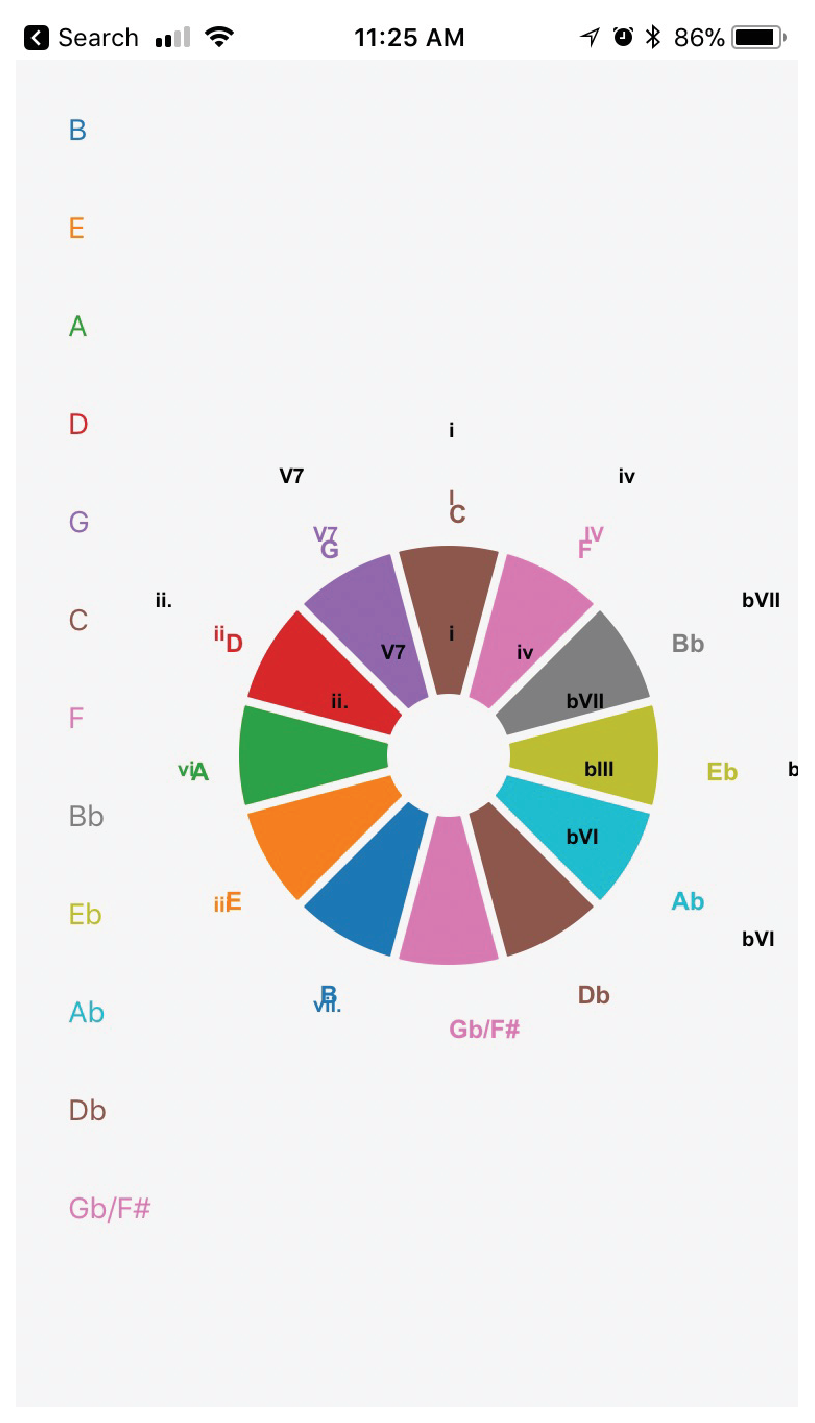
\includegraphics[width=5cm, height=8cm]{circle.eps}
\end{figure}

In this picture you can see an example of what we want the Circle of Fifths to potentially look like.

\subsection{Criteria}

The criteria we defined to determine if the Circle of Fifths is acceptable are listed.
It needs to be easy to make out all of the notes on the circle, it should also be easy to understand the flow from relative key to main key to parallel key on the circle.
The circle should be visually pleasing to the user meaning it matches the rest of the theme and doesn't stand out negatively.

\subsection{Pieces}
\subsubsection{SVG}

Using a vector based graphic that is drawn within the app is one idea we have for implementing the Circle of Fifths.
There are many positives in using a graphic that is actually created within the application's source code.
The main reason being we have more customizability over the animations and interactions with the circle.
Since it is vector based, there will be no issues with resizing the graphic if necessary. 

There are also a lot of different options for creating vector based graphics in React Native.
This is a positive and a negative because the reason there are so many different libraries to help with creating a vector based graphic in React Native is because SVGs aren't supported by the React Native framework itself.
Many people have implemented their own ways of creating these graphics and have put them on the npm registry for others to use, one example is react-native-svg \cite{rnsvg}.
There are many resources and articles out there explaining ways of making svg charts with libraries like ART and d3 such as the article written by David Vacca \cite{rncharts}.
Reading this article brings out some more negatives of the SVG drawing because of the tedious setup required to be able to draw SVGs with the ART library in iOS.
However, the ease of adding animations is evident in the article and is a major positive because our application could be improved with good animations.
We have a simple application so if we can make all interactions and visuals look slick and clean we can make a really nice app.

\subsubsection{Image}

Using images such as .png or .jpeg formatting is another option we have to create the Circle of Fifths segment of our application.
By using an application like Adobe Illustrator or even something as simple as Microsoft Paint we are able to create a circle that looks however we want and is easy to implement in the application.
React Native has a component for images so we can just drop the images in a folder in the source code and load them into the app when an interaction deems an image necessary \cite{rnimage}.
All we need to do then is have a transform property on the image component to rotate it and we have a working application.

Some negatives of the image route of implementation is the fact that for each note positioned at the top of the circle, there will need to be six variations of content.
There needs to be the major key, the minor key, as well as the parallel and relative keys for both of the main keys.
Every combination of those options comes out to six images for each of the 12 notes.
This comes out to 72 images to complete the circle which could potentially take up a lot of space on a phone and is a very clunky implementation for this reason.
To add to this negative, there will also be no way to smoothly animate between images other than a fade in or fade out.
This is because unlike with a vector based graphic where each component is it's own piece of code, the whole image is a piece of code and can't be transformed other than with a rotation of the whole image.

\subsubsection{Ascii}

The last possible implementation we have thought up for the Circle of Fifths is using ascii art.
What this means is using plain text to create a circle and the user can then interact with this text.
The implementation would be very easy since we would be able to use React Native's built in Text component \cite{rntext}.
We would then need to use basic circle geometry to place the text.
We can then group all of the text under one group component and perform rotations on that.
We can also animate text changes because each text component is separated from the group.

The negative to using ascii art or plain text is that it will look very unappealing to the user.
Since our application isn't very complex, sacrificing appearance for ease of implementation may not be the best idea.

\subsection{Discussion}

Overall, it is clear that we have two implementations that are easy to code but have other important limitations.
We also have an implementation that is harder to set up and work with, but this implementation gives us a wide range of customization possibilities.
With an SVG image we can do everything we could possibly want with our circle in terms of appearance and animation, however, since it is not supported by React Native itself we will have difficulties setting up libraries and working with components.
With a normal image we have everything necessary to make a beautiful circle and easily code the interactions, however, we can't interact with specific pieces within the circle and having 72 images in the app takes up an unnecessary amount of space.
Lastly with plain text ascii art we can easily create a circle and interact with specific components within the circle as well as the whole circle, however, the appearance of such a circle looks unprofessional and this can't be ignored.

\subsection{Conclusion}

In conclusion, we have decided to go the SVG vector based graphic route to implement our Circle of Fifths.
We recognize that our application as a whole is not that complex so we can take the time to code and interact with a difficult SVG Circle of Fifths if it will allows us to have the best looking main section of our application.

%%%%%%%%%%%%%%%%%%%

\section{Sidebar Circle of Fifths Implementation}
\subsection{Overview}
Since the main part of our application is the Circle of Fifths page, it is necessary to talk about our implementation of the sidebar for the Circle of Fifths.
The sidebar's main purpose is to show the user the schedule of tonal gravity for the key that is currently selected.
To show the tonal gravity we have decided that the sidebar will be a vertical list of notes where the tonal gravity flows naturally downward.
The second purpose of the sidebar is to alter the contents of the circle, for example, the sidebar should allow the user to change the current key in some manner.
This is where we have multiple ways of implementing the sidebar's functionality.

\begin{figure}[H]
    \centering
    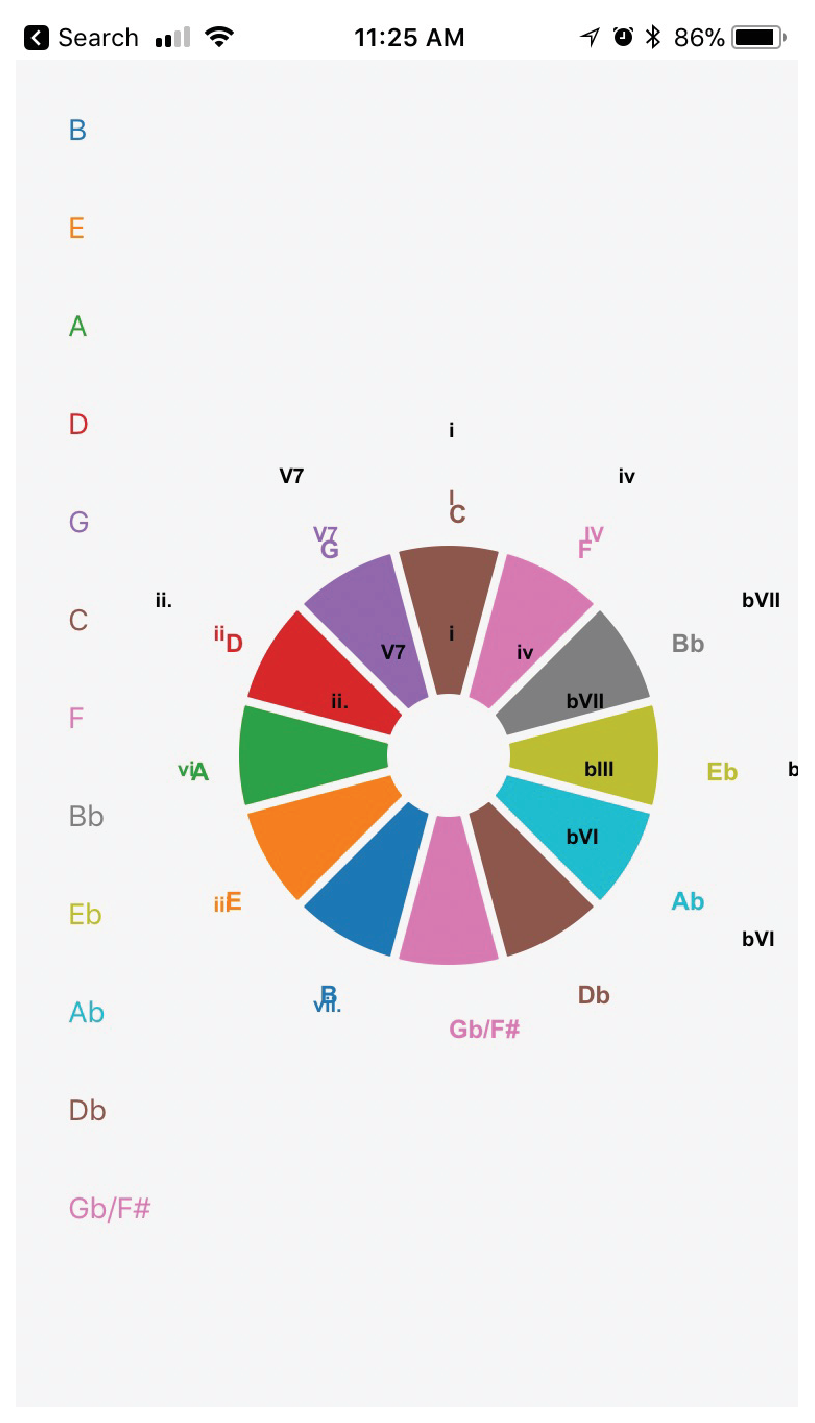
\includegraphics[width=5cm, height=8cm]{circle.eps}
\end{figure}

In this picture you can see an example of what we want the Circle of Fifths' sidebar to potentially look like.

\subsection{Criteria}
The criteria we defined for a working sidebar is the following.
The user should be able to set the main key with the sidebar.
The user should be able to view the tonal gravity of the current key.
The user should be comfortable with the gestures used to alter the circle with the sidebar.

\subsection{Pieces}
\subsubsection{Touchable Notes}

Our first possible implementation is a vertical list of notes where you can select any note and change the contents of the circle.
The change would just be taking whatever note was selected and then moving it to the top of the circle with this note's major key reflected by the chord qualities around the circle.
This is an easy implementation using React Native's Text component.
The Text component has an "onPress" property which allows us to call a function when text is pressed \cite{rntext}.
This is the exact functionality we want because the function we call when a note is pressed can then handle all of the circle transformations.

The negative to having touchable notes is that a single letter of text may be hard for some people to click on and there could be many issues with selecting the wrong note.
Another negative to the touchable notes is that there is not much we can do to transition well from one note's key to another's other than rotating the circle after a click or just resetting the circle immediately after a click.
Rotating might annoy users that want to immediately see the changes reflected, however, immediately changing the circle's contents could also be too abrupt for some users.

\subsubsection{Draggable Bar}

Another implementation is a vertical list of notes where the user can slide their finger from top to bottom on the sidebar and the circle will alter correspondingly.
This is a little more difficult of an implementation but not by much.
We can group the notes which will be made with the React Native Text component with a View component \cite{rnview}.
On this view component we can then have a React Native PanResponder to react to a user's gestures \cite{rnpan}.
In the PanResponder's "onPanResponderMove" function we then include the necessary functionality of altering the circle and we have a complete implementation.

The negative to the draggable bar implementation is that the spacing of the text will determine how easy the dragging gesture is.
If the text is too close together, the dragging will rotate the circle too fast.
However, for most screen sizes, the optimal distance between each note won't be achievable for a really smooth circle and sidebar combination.
Another negative to the draggable bar is that we will need to have a way to lock a note to the top of the circle when the user stops dragging.
This is not a huge negative but it is more implementation that is necessary for the dragging to function correctly.

\subsubsection{Combination of Click and Drag}

The last possible implementation we thought of for the sidebar on our main Circle of Fifths page is to combine both the draggable bar and the touchable note implementations.
Obviously this implementation doubles the amount of work necessary for our team, but there are many positives that come along with this.
The main positive being that users will be able to have options for altering the circle's contents and can end up focusing on one specific implementation based on personal preference.
If one user's fingers are too big to click the notes, they have the option to drag the bar.
If one user likes the dragging animation more than clicking then they can drag.
If a user likes to see their changes reflected on the circle immediately they can click a note.
User's need to be able to be comfortable with our app and giving options on how to use the app would be a big help in achieving comfort.

There is the possibility of the two gestures clashing which could cause problems in the app.
If the implementation is clunky and the gestures are constantly cancelling eachother out, then personal preference doesn't matter because the intended functionality is not truly there.

\subsection{Discussion}

It is clear that there are small issues with all of the implementations listed.
With both the touchable notes and the draggable bar, how the notes are presented play a big part in how effective the implementation is going to be.
The implementation that combines both touching and draggings allows users to decide which implementation is more effective but there is the issue of the gestures cancelling eachother out and causing problems.

\subsection{Conclusion}
In conclusion, we decided to go with the combination of clicking and dragging to give the user the most interaction with the Circle of Fifths.
We can use the PanResponder to implement both implementations instead of using the Text's "onPress" property and this should avoid any overlap between the gestures.
Since the main problem with the combination implementation can be eliminated we decided we should give the user options with how they want to use our application. 

\pagebreak
\bibliography{tech-review}
\bibliographystyle{IEEEtran}

\end{document}